\documentclass[8pt,a4paper,compress]{beamer}

\usepackage{/home/siyer/lib/slides}

\title{Built-in Types of Data}
\date{}

\begin{document}
\begin{frame}
\vfill
\titlepage
\end{frame}

\begin{frame}
\frametitle{Outline}
\tableofcontents
\end{frame}

\section{Types}
\begin{frame}[fragile]
\pause

A data type is set of values and a set of operations defined on those values

\pause
\bigskip

Python supports several built-in data types: \lstinline{int} (for integers), \lstinline{float} (for floating-point numbers), \lstinline{str} (for sequences of characters), \lstinline{bool} (for true/false values), and others

\pause
\bigskip

Python also allows us to compose our own data types, ie, it supports object-oriented programming (OOP)
\end{frame}

\section{Definitions}
\begin{frame}[fragile]
\pause

A literal is a Python-code representation of a data-type value

\pause
\bigskip

For example, \lstinline{1234} and \lstinline{99} are \lstinline{int} literals; \lstinline{3.14159} and \lstinline{2.71828} are \lstinline{float} literals; \lstinline{True} and \lstinline{False} are \lstinline{bool} literals; \lstinline{'Hello, World'} is a \lstinline{str} literal

\pause
\bigskip

An operator is a Python-code representation of a data-type operation

\pause
\bigskip

For example, \lstinline{+} and \lstinline{*} represent addition and multiplication for integers and floating-point numbers; \lstinline{and}, \lstinline{or}, and \lstinline{not} represent boolean operations

\pause
\bigskip

An identifier is a Python-code representation of a name

\pause
\bigskip

Each identifier is a sequence of letters, digits, and underscores, the first of which is not a digit

\pause
\bigskip

For example, \lstinline{abc}, \lstinline{Ab_}, \lstinline{abc123}, and \lstinline{a_b} are valid identifiers, but \lstinline{Ab*}, \lstinline{1abc}, and \lstinline{a+b} are not

\pause
\bigskip

Certain keywords, such as \lstinline{and}, \lstinline{import}, \lstinline{in}, \lstinline{def}, \lstinline{while}, \lstinline{from}, and \lstinline{lambda}, are reserved, and we cannot use them as identifiers; others such as \lstinline{int}, \lstinline{sum}, \lstinline{min}, \lstinline{max}, \lstinline{len}, \lstinline{id}, \lstinline{file}, and \lstinline{input}, have special meaning, so it is best not to use them, either
\end{frame}

\begin{frame}[fragile]
\pause

A variable is a name associated with a data-type value

\pause
\bigskip

For example, the variable \lstinline{total} might represent the running total of a sequence of numbers

\pause
\bigskip

A constant variable describes a variable whose associated data-type value does not change during the execution of a program

\pause
\bigskip

For example, the variable \lstinline{SPEED_OF_LIGHT} might represent the known speed of light

\pause
\bigskip

An expression is a combination of literals, variables, and operators that Python evaluates to produce a value

\pause
\bigskip

For example, \lstinline{4 * (x - 3)} is an expression

\pause
\bigskip

Python has a natural and well-defined set of precedence rules that fully specify the order in which the operators are applied in an expression
\begin{itemize}
\item For arithmetic operations, multiplication and division are performed before addition and subtraction

\item When arithmetic operations have the same precedence, they are left associative, with the exception of the exponentiation operator \lstinline{**}, which is right associative

\item We can use parentheses to override precedence rules
\end{itemize} 
\end{frame}

\begin{frame}[fragile]
\pause

We use an assignment statement to define a variable and associate it with a data-type value
\begin{lstlisting}[language={}]
<variable> = <value>
\end{lstlisting}

\pause
\bigskip

For example, the statement 
\begin{lstlisting}[language=Python]
a = 1234
\end{lstlisting}
defines an identifier \lstinline{a} to be a new variable and associates it with the integer data-type value \lstinline{1234}

\pause
\bigskip

To represent the absence of a value, we can use the value \lstinline{None}

\pause
\bigskip

All data values in Python are represented by objects, each characterized by its identity (or memory address), type, and value

\pause
\bigskip

For example, the following figure shows how the variable \lstinline{a} as defined above, might be represented in memory (left) and conceptually (right) 
\begin{center}
\visible<6->{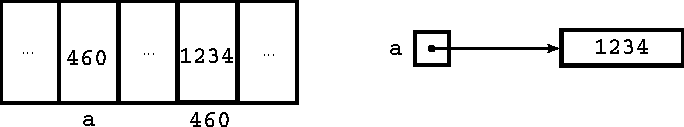
\includegraphics[scale=0.6]{figures/object_representation.pdf}}
\end{center}
\end{frame}

\begin{frame}[fragile]
Consider the following code that exchanges \lstinline{a = 1234} and \lstinline{b = 99} (more precisely, the objects bound to \lstinline{a} and \lstinline{b})

\begin{lstlisting}[language=Python]
t = a
a = b
b = t
\end{lstlisting}

\pause
\bigskip

The object-level trace for the code is shown below
\begin{center}
\visible<2->{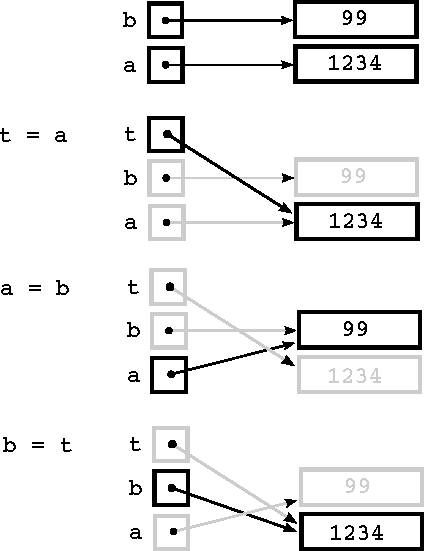
\includegraphics[scale=0.6]{figures/object_level_trace.pdf}}
\end{center}
\end{frame}

\section{Strings}
\begin{frame}[fragile]
\pause

The \lstinline{str} data type represents strings (sequences of characters), for use in text processing

\pause
\bigskip

A \lstinline{str} literal is specified by enclosing a sequence of characters in matching single quotes

\pause
\bigskip

For example, \lstinline{'ab'} is a \lstinline{str} literal

\pause
\bigskip

We can specify tab, newline, backslash, and single quote characters using escape sequences \lstinline{'\t'}, \lstinline{'\n'}, \lstinline{'\\'}, and \lstinline{'\''}, respectively

\pause
\bigskip

We can concatenate two strings using the \lstinline{+} operator

\pause
\bigskip

For example, the expression \lstinline{'123' + '456'} evaluates to the \lstinline{str} object whose value is \lstinline{'123456'}

\pause
\bigskip

We can multiply a \lstinline{str} object $s$ by a number $n$ to obtain a \lstinline{str} object whose value is the string $s$ repeated $n$ times

\pause
\bigskip

For example, the expressions \lstinline{3 * 'ab'} and \lstinline{'ab' * 3} evaluate to the \lstinline{str} object whose value is \lstinline{'ababab'}

\pause
\bigskip

The \lstinline{str} data type

\begin{center}
\begin{tabular}{c|c}
values & sequences of characters \\ 
typical literals & \lstinline$'Hello, World'$, \lstinline$'Python\'s'$ \\ 
operations & concatenate, multiply \\
operators & \lstinline$+$, \lstinline$*$
\end{tabular} 
\end{center}
\end{frame}

\begin{frame}[fragile]
\pause

\begin{framed}
\tiny ruler.py: The ruler function $R(n)$ is the exponent of the largest power of 2 which 
divides $2n$. The $i$th row in the output lists the values of $R(n)$ for $n=1,2,
\dots,2^i-1$.
\end{framed}

\begin{lstlisting}[language=Python]
import stdio

ruler1 = '1'
ruler2 = ruler1 + ' 2 ' + ruler1
ruler3 = ruler2 + ' 3 ' + ruler2
ruler4 = ruler3 + ' 4 ' + ruler3
stdio.writeln(ruler1)
stdio.writeln(ruler2)
stdio.writeln(ruler3)
stdio.writeln(ruler4)
\end{lstlisting}

\pause

\begin{lstlisting}[language={}]
$ python3 ruler.py 
1
1 2 1
1 2 1 3 1 2 1
1 2 1 3 1 2 1 4 1 2 1 3 1 2 1
\end{lstlisting}
\end{frame}

\begin{frame}[fragile]
\pause

The built-in function \lstinline{str()} can be used to convert numbers into strings

\pause
\bigskip

For example, \lstinline{str(123)} evaluates to the \lstinline{str} object \lstinline{'123'}, and \lstinline{str(123.45)} evaluates to the \lstinline{str} object \lstinline{'123.45'}

\pause
\bigskip

The built-in functions \lstinline{int()} and \lstinline{float()} can be used to convert strings to numbers

\pause
\bigskip

For example, \lstinline{int('123')} is equivalent to the \lstinline{int} literal \lstinline{123}, and \lstinline{float('123.45')} is equivalent to the \lstinline{float} literal \lstinline{123.45}
\end{frame}

\section{Integers}
\begin{frame}[fragile]
\pause

The \lstinline{int} data type represents integers or natural numbers

\pause
\bigskip

We can specify an \lstinline{int} literal with a sequence of digits \lstinline{0} through \lstinline{9}

\pause
\bigskip

Python includes operators for common arithmetic operations on integers, including \lstinline{+} for addition, \lstinline{-} for subtraction, \lstinline{*} for multiplication, \lstinline{//} for floored division, \lstinline{%} for remainder, and \lstinline{**} for exponentiation

\pause
\bigskip

The \lstinline{int} data type
\begin{center}
\begin{tabular}{c|c}
values & integers \\
typical literals & \lstinline$1234$, \lstinline$99$, \lstinline$0$, \lstinline$1000000$ \\ 
operations & sign, add, subtract, multiply, floored divide, remainder, power \\
operators & \lstinline$+$ \lstinline$-$, \lstinline$+$, \lstinline$-$, \lstinline$*$, \lstinline$//$, \lstinline$%$, \lstinline$**$
\end{tabular} 
\end{center}
\end{frame}

\begin{frame}[fragile]
\pause

\begin{framed}
\tiny intops.py: Accept two integers $a$ and $b$ as command-line arguments, perform integer operations on them, and write the results to standard output.
\end{framed}

\begin{lstlisting}[language=Python]
import stdio
import sys

a = int(sys.argv[1])
b = int(sys.argv[2])
total = a +  b
diff  = a -  b
prod  = a *  b
quot  = a // b
rem   = a %  b
exp   = a ** b
stdio.writeln(str(a) + ' +  ' + str(b) + ' = ' + str(total))
stdio.writeln(str(a) + ' -  ' + str(b) + ' = ' + str(diff))
stdio.writeln(str(a) + ' *  ' + str(b) + ' = ' + str(prod))
stdio.writeln(str(a) + ' // ' + str(b) + ' = ' + str(quot))
stdio.writeln(str(a) + ' %  ' + str(b) + ' = ' + str(rem))
stdio.writeln(str(a) + ' ** ' + str(b) + ' = ' + str(exp))
\end{lstlisting}

\pause

\begin{lstlisting}[language={}]
$ python3 intops.py 1234 5
1234 +  5 = 1239
1234 -  5 = 1229
1234 *  5 = 6170
1234 // 5 = 246
1234 %  5 = 4
1234 ** 5 = 2861381721051424
\end{lstlisting}
\end{frame}

\section{Floating-point Numbers}
\begin{frame}[fragile]
\pause

The \lstinline{float} data type represents floating-point numbers, for use in scientific and commercial applications

\pause
\bigskip

We can specify a floating-point literal using a sequence of digits with a decimal point

\pause
\bigskip

For example, \lstinline{3.14159} is a \lstinline{float} literal that represents an approximation to $\pi$

\pause
\bigskip

Alternatively, we can use a notation similar to scientific notation: the literal \lstinline{6.022e23} represents the number $6.022 \times 10^{23}$

\pause
\bigskip

Python includes operators for common arithmetic operations on floating-point numbers, including \lstinline{+} for addition, \lstinline{-} for subtraction, \lstinline{*} for multiplication, \lstinline{/} for division, and \lstinline{**} for exponentiation

\pause
\bigskip

The \lstinline{float} data type
\begin{center}
\begin{tabular}{c|c}
values & real numbers \\
typical literals & \lstinline$3.14159$, \lstinline$6.022e23$, \lstinline$2.0$, \lstinline$1.4142135623730951$ \\ 
operations & sign, add, subtract, multiply, divide, power \\
operators & \lstinline$+$ \lstinline$-$, \lstinline$+$, \lstinline$-$, \lstinline$*$, \lstinline$/$, \lstinline$**$
\end{tabular} 
\end{center}
\end{frame}

\begin{frame}[fragile]
\pause

\begin{framed}
\tiny floatops.py: Accept two floats $a$ and $b$ as command-line arguments, perform floating-point operations on them, and write the results to standard output.
\end{framed}

\begin{lstlisting}[language=Python]
import stdio
import sys

a = float(sys.argv[1])
b = float(sys.argv[2])
total = a + b
diff  = a - b
prod  = a * b
quot  = a / b
exp   = a ** b
stdio.writeln(str(a) + ' +  ' + str(b) + ' = ' + str(total))
stdio.writeln(str(a) + ' -  ' + str(b) + ' = ' + str(diff))
stdio.writeln(str(a) + ' *  ' + str(b) + ' = ' + str(prod))
stdio.writeln(str(a) + ' /  ' + str(b) + ' = ' + str(quot))
stdio.writeln(str(a) + ' ** ' + str(b) + ' = ' + str(exp))
\end{lstlisting}

\pause

\begin{lstlisting}[language={}]
$ python3 floatops.py 123.456 78.9
123.456 +  78.9 = 202.356
123.456 -  78.9 = 44.556
123.456 *  78.9 = 9740.6784
123.456 /  78.9 = 1.5647148289
123.456 ** 78.9 = 1.04788279167e+165
\end{lstlisting}
\end{frame}

\begin{frame}[fragile]
\pause

\begin{framed}
\tiny quadratic.py: Accept floats $b$ and $c$ as command-line arguments, compute the the roots of the polynomial $x^2 + bx + c$ using the quadratic formula $x=(-b\pm \sqrt{b^2-4c})/2$, and write the roots to standard output.
\end{framed}

\begin{lstlisting}[language=Python]
import math
import stdio
import sys

b = float(sys.argv[1])
c = float(sys.argv[2])
discriminant = b * b - 4.0 * c
d = math.sqrt(discriminant)
stdio.writeln((-b + d) / 2.0)
stdio.writeln((-b - d) / 2.0)
\end{lstlisting}

\pause

\begin{lstlisting}[language={}]
$ python3 quadratic.py -3.0 2.0
2.0
1.0
$ python3 quadratic.py -1.0 -1.0
1.61803398875
-0.61803398875
$ python quadratic.py 1.0 1.0
Traceback (most recent call last):
  File "quadratic.py", line 17, in <module>
    d = math.sqrt(discriminant)
ValueError: math domain error
\end{lstlisting}
\end{frame}

\section{Booleans}
\begin{frame}[fragile]
\pause

The \lstinline{bool} data type represents truth values (true or false) from logic 

\pause
\bigskip

The two \lstinline{bool} literals are represented as \lstinline{True} and \lstinline{False}

\pause
\bigskip

The operators defined for \lstinline{bool} objects, namely \lstinline{and}, \lstinline{or}, and \lstinline{not}, are known as logical operators, and having the following truth tables

\begin{center}
\begin{tabular}{cc|c}
\lstinline$x$ & \lstinline$y$ & \lstinline$x and y$ \\ \hline
\lstinline$False$ & \lstinline$False$ & \lstinline$False$ \\
\lstinline$False$ & \lstinline$True$ & \lstinline$False$ \\
\lstinline$True$ & \lstinline$False$ & \lstinline$False$ \\
\lstinline$True$ & \lstinline$True$ & \lstinline$True$
\end{tabular}\hspace{1cm} \begin{tabular}{cc|c}
\lstinline$x$ & \lstinline$y$ & \lstinline$x or y$ \\ \hline
\lstinline$False$ & \lstinline$False$ & \lstinline$False$ \\
\lstinline$False$ & \lstinline$True$ & \lstinline$True$ \\
\lstinline$True$ & \lstinline$False$ & \lstinline$True$ \\
\lstinline$True$ & \lstinline$True$ & \lstinline$True$
\end{tabular}\hspace{1cm} \begin{tabular}{c|c}
\lstinline$x$ & \lstinline$not x$ \\ \hline
\lstinline$False$ & \lstinline$True$ \\
\lstinline$True$ & \lstinline$False$
\end{tabular}
\end{center}

\pause
\bigskip

The \lstinline{bool} data type

\begin{center}
\begin{tabular}{c|c}
values & true, false \\ 
typical literals & \lstinline$True$, \lstinline$False$ \\ 
operations & and, or, not \\
operators & \lstinline$and$, \lstinline$or$, \lstinline$not$
\end{tabular} 
\end{center}
\end{frame}

\begin{frame}[fragile]
\pause

The comparison operators \lstinline{==}, \lstinline{!=}, \lstinline{<}, \lstinline{<=}, \lstinline{>}, \lstinline{>=}, \lstinline{is}, and \lstinline{is not} are defined for both integers and floats, and evaluate to a boolean result

\pause
\bigskip

For example, \lstinline{2 == 2} evaluates to \lstinline{True}, \lstinline{2 == 3} evaluates to \lstinline{False}, \lstinline{2 < 13} evaluates to \lstinline{True} 

\pause
\bigskip

Comparison operators have lower precedence than arithmetic operators and higher precedence than boolean operators, so you do not need the parentheses in an expression like \lstinline{(b * b - 4.0 * a * c) >= 0.0}
\end{frame}

\begin{frame}[fragile]
\pause

\begin{framed}
\tiny leapyear.py: Accept an integer $year$ as command-line argument, and write \lstinline{True} to standard output if $year$ is a leap year and \lstinline{False} otherwise. A year is a leap year if it is divisible by 4 \emph{and} not divisible by 100 \emph{or} is divisible by 400.
\end{framed}

\begin{lstlisting}[language=Python]
import stdio
import sys

year = int(sys.argv[1])
isLeapYear = (year % 4 == 0)
isLeapYear = isLeapYear and (year % 100 != 0)
isLeapYear = isLeapYear or  (year % 400 == 0)
stdio.writeln(isLeapYear)
\end{lstlisting}

\pause

\begin{lstlisting}[language={}]
$ python3 leapyear.py 2016
True
$ python3 leapyear.py 1900
False
$ python3 leapyear.py 2000
True
\end{lstlisting}
\end{frame}

\section{Functions and APIs}
\begin{frame}[fragile]
\pause

Many programming tasks involve not only built-in operators, but also functions

\pause
\bigskip

We consider three kinds of functions
\begin{enumerate}
\item Built-in functions (such as \lstinline{int()}, \lstinline{float()}, and \lstinline{str()}) that you can use directly in any Python program

\item Standard functions (such as \lstinline{math.sqrt()}) that are defined in a Python standard module and are available in any program that imports the module

\item User-defined functions (such as \lstinline{stdio.write()} and \lstinline{stdio.writeln()}) that are defined in third-party modules
\end{enumerate}

\pause
\bigskip

We can call a function in our code by typing its name followed by arguments (which are just expressions), enclosed in parentheses and separated by commas

\pause
\bigskip

For example, \lstinline{math.sqrt(2.0)} is a function call

\pause
\bigskip

When Python executes your program, we say that it calls (or evaluates) the function with the given arguments.

\pause
\bigskip

A function call that returns a value is an expression, so we can use it in the same way that we use variables and literals to build up more complicated expressions

\pause
\bigskip

For example, \lstinline{math.sin(x) * math.cos(y)} is an expression

\pause
\bigskip

A function call that does not return a value, but has a side effect, can only be used as a statement

\pause
\bigskip

For example, \lstinline{stdio.writeln('Hello, World')} is a statement
\end{frame}

\begin{frame}[fragile]
\pause

We summarize functions in a table called the application programming interface (API)

\pause
\bigskip

Built-in functions

\begin{center}
\begin{tabular}{cc}
function & description \\ \hline
\lstinline$abs(x)$ & absolute value of $x$ \\
\lstinline$max(a, b)$ & maximum value of $a$ and $b$ \\
$\dots$ & $\dots$
\end{tabular} 
\end{center}

\pause
\smallskip

Standard functions from Python's \lstinline{math} and \lstinline{random} modules

\begin{center}
\begin{tabular}{cc}
function & description \\ \hline
\lstinline$math.sin(x)$ & sine of $x$ (expressed in radians) \\
\lstinline$math.cos(x)$ & cosine of $x$ (expressed in radians) \\
$\dots$ & $\dots$
\end{tabular} 

\begin{tabular}{cc}
function & description \\ \hline
\lstinline$random.random()$ & a random float from the real interval $[0, 1)$ \\
\lstinline$random.randrange(x, y)$ & a random integer from the integer interval $[x, y)$ \\
$\dots$ & $\dots$
\end{tabular} 
\end{center}

\pause
\smallskip

User-defined functions from the \lstinline{stdio} module

\begin{center}
\begin{tabular}{cc}
function & description \\ \hline
\lstinline$stdio.write(x)$ & write $x$ to standard output \\
\lstinline$stdio.writeln(x)$ & write $x$ to standard output, followed by a newline \\
$\dots$ & $\dots$
\end{tabular} 
\end{center}
\end{frame}

\section{Type Conversion}
\begin{frame}[fragile]
\pause

We can use built-in functions \lstinline{int()}, \lstinline{float()}, \lstinline{str()}, and \lstinline{round()} to explicitly convert from strings to integers or floats, and vice versa

\pause
\bigskip

Python also supports implicit conversion (aka automatic promotion or coercion)

\pause
\bigskip

For example, we can use an integer where a float is expected, as in \lstinline{math.sqrt(4)}, which evaluates to \lstinline{2.0}
\end{frame}

\section{Interactive Python}
\begin{frame}[fragile]
\pause

We can use Python as a calculator by the running command \lstinline{python3} in the terminal

\begin{lstlisting}[language={}]
$ python3
...
>>> 1 + 2
3
>>> a = 1
>>> b = 2
>>> a + b
3
>>> import math
>>> math.sqrt(2.0)
1.4142135623730951
>>> math.e
2.718281828459045
\end{lstlisting}

\pause
\bigskip

We can type \lstinline{dir()} without arguments to get a list of names in the current local scope; With an object argument, we get a list of valid attributes for that object
\begin{lstlisting}[language={}]
>>> dir()
['__builtins__', '__doc__', '__name__', '__package__', 'a', 'b', 'math']
>>> dir(math)
['__doc__', '__name__', '__package__', 'acos', 'acosh', 'asin', 'asinh', 'atan', 
'atan2', 'atanh', 'ceil', 'copysign', 'cos', 'cosh', 'degrees', 'e', 'erf', 
'erfc', 'exp', 'expm1', 'fabs', 'factorial', 'floor', 'fmod', 'frexp', 'fsum', 
'gamma', 'hypot', 'isinf', 'isnan', 'ldexp', 'lgamma', 'log', 'log10', 'log1p', 
'modf', 'pi', 'pow', 'radians', 'sin', 'sinh', 'sqrt', 'tan', 'tanh', 'trunc']
>>> 
\end{lstlisting}
\end{frame}

\begin{frame}[fragile]
\pause

We can type \lstinline{help()} to get access to Python's extensive interactive documentation
\begin{lstlisting}[language={}]
>>> help(math)

Help on built-in module math:

NAME
    math

FILE
    (built-in)

DESCRIPTION
    This module is always available.  It provides access to the
    mathematical functions defined by the C standard.

FUNCTIONS
    acos(...)
        acos(x)
        
        Return the arc cosine (measured in radians) of x.
...
DATA
    e = 2.718281828459045
    pi = 3.141592653589793
\end{lstlisting}

\pause
\bigskip

We can type \lstinline{exit()} to return to the terminal
\begin{lstlisting}[language={}]
>>> exit()
$
\end{lstlisting}
\end{frame}
\end{document}
